\documentclass[preprint,12pt]{elsarticle}

\usepackage{amsmath,amssymb}
\usepackage{booktabs}
\usepackage{graphicx}
\usepackage{natbib}
\usepackage{url}
\usepackage{array}
\def\UrlBreaks{\do\/\do-\do\_}
\emergencystretch=2em

\graphicspath{{../results/paper_figures/}{../results/audit_case/fashion_noniid_signflip_proposed_s42/}}

\begin{document}

\begin{frontmatter}

\title{Validator-Backed Auditable Robust Aggregation for Trustworthy Federated Learning}

\author[aff1]{Shiqi Huang\corref{cor1}}
\ead{shiqihuang666@gmail.com}
\address[aff1]{Faculty of Computational Mathematics and Cybernetics, Lomonosov Moscow State University, Moscow, Russia}
\cortext[cor1]{Corresponding author.}

\begin{abstract}
Federated learning enables collaborative model training without centralizing raw data, but the learning process remains vulnerable to poisoning attacks and opaque aggregation decisions made by a single service operator. Existing robust aggregation rules reduce malicious update influence, yet they usually assume faithful server execution and provide limited evidence for explaining why a client was accepted, down-weighted, or rejected. This paper proposes a validator-backed auditable robust aggregation framework for trustworthy federated learning under client poisoning and aggregator-side tampering. The learning rule scores client updates using magnitude deviation, directional consistency, and historical stability, combines the score with smoothed reputation, and performs dynamic weighted aggregation under heterogeneous data. To make learning decisions verifiable, the selected aggregator proposes anomaly scores, reputation updates, aggregation weights, model hashes, and commitment-bound evidence; permissioned validators independently recompute the deterministic mapping from evidence to decisions before threshold finality. Thus, the aggregation decision itself becomes an independently checked learning-system object. Experiments on Fashion-MNIST and CIFAR-10 cover IID and Dirichlet Non-IID settings under sign-flip, adaptive-scaling, backdoor, and collusive-direction attacks, with FLTrust and FLAME-style extensions, malicious-ratio tests, and ablations. The method avoids the FedAvg failure modes observed in attacked settings, maintains low attack success rate, and remains competitive with strong robust baselines. Audit and validator experiments show reconstructable recorded decisions, rejection of tested invalid aggregation proposals under the default honest-validator setting, explicit Byzantine and dropout boundaries, accountable invalid-signing evidence, and modest verification overhead.
\end{abstract}

\begin{keyword}
trustworthy federated learning \sep robust aggregation \sep poisoning attack \sep auditable learning systems \sep reputation-aware aggregation \sep validator-backed verification \sep model poisoning defense
\end{keyword}

\end{frontmatter}

\section*{Abbreviations}

\begin{tabular}{ll}
ASR & Attack success rate \\
BFT & Byzantine fault tolerance \\
DFL & Decentralized federated learning \\
FL & Federated learning \\
IID & Independent and identically distributed \\
IoT & Internet of Things \\
Non-IID & Non-independent and non-identically distributed \\
RTT & Round-trip time \\
\end{tabular}

\section{Introduction}

Federated learning (FL) allows multiple clients to collaboratively train a global model while keeping raw data local \citep{mcmahan2017fedavg,kairouz2021advances}. It is now a core learning paradigm for data-distributed environments such as mobile intelligence, edge learning, industrial Internet-of-Things analytics, healthcare consortia, and cross-organization machine learning. This setting has motivated production-scale FL systems and heterogeneity-aware optimization methods \citep{bonawitz2019scale,li2020fedprox,karimireddy2020scaffold,reddi2021fedopt}. From a trustworthy learning perspective, however, conventional server-mediated FL replaces centralized data collection with a new trust boundary: the aggregation service must process updates from clients that may be faulty, compromised, or strategically malicious, while the parties affected by aggregation decisions often receive little evidence explaining how those decisions were made.

This trust boundary creates three linked security problems. First, malicious clients can manipulate uploaded model updates to degrade global accuracy, trigger targeted misclassification, or bypass defenses that assume poisoned updates are simple outliers \citep{fang2020local,bagdasaryan2020backdoor,baruch2019little,cao2021fltrust}. Classical robust aggregation rules, including Krum, coordinate-wise Median, Trimmed Mean, Bulyan, and geometric median, were designed to tolerate Byzantine clients by filtering or reducing the effect of abnormal updates \citep{blanchard2017krum,yin2018byzantine,elmhamdi2018bulyan,pillutla2022rfa}. Second, Non-IID data make this filtering problem ambiguous because honest client updates may naturally differ from one another. A defense that rejects every unusual update can suppress useful minority-client information, whereas a defense that tolerates too much heterogeneity gives adaptive attackers room to hide.

Third, robustness alone is not sufficient for trustworthy FL because the entity that computes the aggregate may itself become part of the trust problem. When a client update is rejected or assigned a near-zero aggregation weight, the system should preserve the evidence behind that decision so that operators can reconstruct the training process, diagnose attacks, and audit whether benign heterogeneous clients were unfairly suppressed. Blockchain-assisted and decentralized FL have been proposed to improve transparency, coordination, incentive compatibility, and accountability \citep{lu2020blockchain,nguyen2021blockchainedge,dong2024blockchain,zhang2024bitfl,ren2024bpfl,awan2022blockchainflsurvey,yuan2024dflsurvey,jiang2023blockflsurvey}. Nevertheless, simply recording model hashes or training metrics does not make the learning decision trustworthy, and a hash chain controlled by the same aggregation server does not protect against aggregator-side insider manipulation. The audit layer is useful only if the evidence behind the aggregation decision is checked by parties other than the proposer before it becomes part of the finalized record.

This requirement is practical rather than merely diagnostic. In multi-party FL deployments such as cross-institutional analytics, industrial Internet of Things, and collaborative edge intelligence, operators may need to investigate security incidents, justify client exclusion, and demonstrate that model-governance rules were applied consistently. A defense that only outputs a final aggregate provides limited support for this type of trustworthy learning accountability.

To address these issues, this paper proposes a permissioned validator-backed auditable robust aggregation framework for trustworthy FL. The aggregation rule evaluates client updates through multiple signals so that norm outliers, directional inconsistency, and unstable history are not treated as interchangeable evidence. The audit layer separates proposal from finalization: a round-specific aggregator proposes anomaly scores, reputation changes, aggregation weights, and model hashes, but the proposal is finalized only after independent validators verify the evidence and produce threshold signatures. Instead of permanently accepting or rejecting clients using a static threshold, the framework assigns dynamic aggregation weights based on both current anomaly scores and historical trust. This design targets a specific learning-system objective: keeping the global model competitive under poisoning while making each aggregation decision reconstructable and resistant to unilateral manipulation by a dishonest aggregator under stated committee assumptions.

The main contributions are:
\begin{enumerate}
  \item We design a reputation-aware robust aggregation rule for heterogeneous FL that combines norm deviation, directional consistency, history stability, smoothed trust, hard rejection, and dynamic weighting.
  \item We formulate aggregation decisions as verifiable learning-system objects: anomaly scores, reputation updates, aggregation weights, commitments, model hashes, and evidence hashes must be independently recomputable before an audit record can be finalized.
  \item We introduce a validator-backed audit mechanism that records aggregation evidence and prevents a single aggregator from unilaterally finalizing manipulated decision records when the threshold assumption holds.
  \item We provide a reproducible evaluation that links model robustness, component ablation, decision auditability, validator-fault boundaries, accountability evidence, liveness, scalability, and overhead to the same trustworthy-FL argument.
\end{enumerate}

The evaluation is organized around the same argument chain. Main robustness experiments test whether the aggregation rule remains useful under poisoning. Extension and collusive-direction experiments test whether the method remains competitive against trust-root, backdoor-specific, and coordinated-adversary settings while exposing its high-adversary-fraction boundary. Sensitivity and ablation studies test whether the scoring weights and components are necessary. Auditability experiments test whether aggregation decisions can be reconstructed after training. Validator experiments test whether a dishonest aggregator can finalize manipulated evidence and where the committee fault and liveness boundaries lie. Cost and scalability experiments then quantify the additional local verification work, proposal sizes, committee communication, estimated finality latency, and event-driven threshold-finality behavior introduced by validator-backed audit finality.

\section{Related Work}

\subsection{Federated Learning Robustness Under Heterogeneity}

FedAvg established a communication-efficient training paradigm for decentralized data \citep{mcmahan2017fedavg}, and subsequent work has clarified that FL differs from conventional distributed optimization because clients are statistically and systemically heterogeneous \citep{kairouz2021advances}. FedProx, SCAFFOLD, and adaptive federated optimization address optimization drift rather than poisoning, but they motivate the emphasis on Non-IID data because benign updates may naturally deviate from the global mean \citep{li2020fedprox,karimireddy2020scaffold,reddi2021fedopt}. Poisoning and backdoor attacks exploit this ambiguity by manipulating data, labels, or uploaded model updates while attempting to preserve apparent plausibility \citep{fang2020local,bagdasaryan2020backdoor,baruch2019little,xie2020dba,nguyen2022flame}.

Robust aggregation methods such as Krum, Median, Trimmed Mean, Bulyan, and geometric median reduce the influence of abnormal updates \citep{blanchard2017krum,yin2018byzantine,elmhamdi2018bulyan,pillutla2022rfa}. Trust-based and backdoor-specific defenses add complementary signals: FLTrust uses a trusted reference update, FoolsGold exploits persistent similarity, and FLAME combines clustering, clipping, and noise injection \citep{cao2021fltrust,fung2020foolsgold,nguyen2022flame}. Recent adaptive and history-aware defenses further show that single-signal filtering is often insufficient under heterogeneous and adaptive attacks \citep{wang2025adaaggrl,wang2025fedhan}. These works motivate the paper's multi-signal aggregation rule and the separate treatment of trust assumptions across baselines.

\subsection{Auditable and Validator-Assisted Federated Learning}

Auditable FL mechanisms use ledgers, committees, or decentralized coordination to reduce dependence on a single trusted server and to preserve evidence about training decisions. Early decentralized and blockchain-assisted FL prototypes such as Biscotti, BLADE-FL, and BlockDFL explore ledger-based coordination for model exchange, incentive handling, or server-trust reduction \citep{shayan2018biscotti,li2021bladefl,qin2022blockdfl}. Recent surveys further identify topology, communication, privacy, data heterogeneity, trust management, and compatibility overhead as central challenges for decentralized and ledger-assisted FL \citep{yuan2024dflsurvey,jiang2023blockflsurvey,hallaji2024dflsecurity}. Peer-reviewed auditable-FL defenses have also begun to connect ledger records with poisoning detection and robust aggregation \citep{dong2024blockchain,zhang2024bitfl,ren2024bpfl}, while newer preprints investigate validator-, consensus-, and clustering-based variants \citep{garcia2025kfc,carney2025fidelis,bouchiha2026abc}.

Committee-based designs are particularly relevant. BFLC uses committee consensus to reduce finality cost in blockchain-based FL, while VBFL introduces validator-based local-model validation and proof-of-stake-inspired consensus \citep{li2020bflc,chen2021vbfl}. These designs motivate a validator role that is not limited to record storage but can also check model or update legitimacy. At the same time, classical BFT systems such as PBFT, HotStuff, Tendermint, and Hyperledger Fabric show that replicated finality requires explicit fault assumptions, membership or leader rules, communication procedures, and implementation choices \citep{castro1999pbft,yin2019hotstuff,buchman2018tendermint,androulaki2018fabric}. Survey and benchmarking work further emphasizes that safety, liveness, and throughput depend on validator availability and communication overhead \citep{zhang2022bftsurvey,alqahtani2021bottlenecks}. Committee selection also creates security questions, including Sybil resistance, validator collusion, and static-committee capture \citep{rajab2020sybil}. The present work therefore focuses on a narrower learning-system point: making robust aggregation decisions independently verifiable before they are finalized into an audit chain, while leaving production-grade consensus networking as deployment work.

\subsection{Research Gap}

Existing robust aggregation rules mainly optimize the current-round aggregate, while audit-assisted FL often treats the ledger or record layer as storage, incentive, or coordination infrastructure. These two lines of work are complementary but not tightly coupled. A rejected or down-weighted update should be explainable after training: the system should record which anomaly signals were observed, how reputation changed, and how those signals affected the final aggregation weight. More importantly, if the aggregator itself may be dishonest, audit evidence cannot be finalized solely by that same aggregator. The gap addressed in this paper is therefore the missing verification layer between robust aggregation and audit finality. The contribution is to treat the aggregation decision itself as a verifiable learning-system object: client commitments, anomaly evidence, reputation updates, aggregation weights, model hashes, aggregator authorization, validator votes, and hash linkage are bound into a threshold-finalized record. This coupling makes robustness decisions operational during training and independently reconstructable afterward, while making clear that production-grade consensus networking remains a deployment layer around the FL-specific validity predicate.

Table~\ref{tab:positioning} summarizes this positioning. The paper is not another pure robust aggregator, because it evaluates whether the evidence behind the aggregate can be reconstructed and independently verified. It is also not merely an audit-log design, because validators recompute the aggregation decision rather than only storing hashes or metrics. Compared with committee-consensus FL designs, the focus is narrower but more specific: defining and evaluating the FL aggregation-decision validity predicate that a committee must check before finality.

\begin{table}[t]
\centering
\caption{Positioning of the proposed work relative to robust, auditable, and validator-assisted FL directions.}
\label{tab:positioning}
\resizebox{\linewidth}{!}{%
\begin{tabular}{llll}
\toprule
Direction & Main objective & Typical limitation for this paper's threat model & This paper's distinction \\
\midrule
Robust aggregation & Reduce malicious update influence & Aggregator execution and audit trail are trusted & Adds validator-verified decision evidence \\
Trust/backdoor defenses & Use trusted data, similarity, clustering, or clipping & Often tied to specific trust or attack assumptions & Reports separately under stated assumptions \\
Audit logging for FL & Store hashes, models, metrics, or incentives & Logged values may be wrong if proposer is dishonest & Validators recompute scores and weights before finality \\
Committee-assisted FL & Reduce finality cost or validate local models & Often focuses on consensus or model acceptance & Verifies the aggregation-decision predicate itself \\
BFT finality layers & Replicate ordering/finality under system assumptions & Consensus does not define FL-specific validity & Provides the application validity rule for such finality layers \\
\bottomrule
\end{tabular}}
\end{table}

\section{Threat Model and Problem Definition}

We consider a permissioned consortium FL system with $N$ clients, a set of eligible round aggregators, and a validator committee $\mathcal{V}$ of size $m$. At communication round $t$, the current global model parameters $w_t$ are made available to selected clients. Client $i$ trains locally on its private dataset $D_i$ and returns a local model $w_{t,i}$ or, equivalently, an update vector
\begin{equation}
u_{t,i}=\mathrm{vec}(w_{t,i}-w_t),
\end{equation}
where $\mathrm{vec}(\cdot)$ denotes concatenation of all floating-point model parameters. Client $i$ has $n_i=|D_i|$ training samples. A subset $\mathcal{M}_t$ of clients may be malicious. Malicious clients can poison uploaded model updates, collude with each other, and adapt update magnitudes to evade simple norm-based thresholds.

The aggregation role is not assumed to be permanently trusted. A public leader-selection rule chooses a round aggregator for each round. The selected aggregator proposes anomaly scores, reputation updates, aggregation weights, model hashes, and an audit payload. A dishonest aggregator may alter scores, change aggregation weights, omit clients, introduce fake clients, modify model hashes, equivocate across proposals, or attempt to finalize a self-serving audit record. The aggregator can propose a block but cannot finalize it alone.

Validators are permissioned entities that verify proposed audit blocks. In the intended consortium setting, the validator set can be formed from independent organizations, institutional audit nodes, edge-service operators, or governance members rather than from the same administrative domain as the round aggregator. The committee may be fixed for a deployment epoch or periodically rotated by an external governance rule. This paper does not claim to solve permissionless validator admission, Sybil resistance, stake economics, or committee election; instead, it evaluates what a given permissioned committee must verify before finalizing an FL aggregation decision. A block is finalized only if at least $q$ validators sign it. We consider Byzantine validators that may sign invalid proposals and offline validators that do not respond. The protocol's safety is meaningful when fewer than $q$ validators sign an invalid proposal; if $q$ Byzantine or lazy validators collude to sign an invalid proposal, threshold finality can be subverted, although the signatures provide accountability evidence. Liveness requires at least $q$ available validators. This work therefore claims threshold-finalized auditability under explicit committee assumptions, not unconditional security against validator-majority collusion or permissionless Sybil attacks. Supplementary Table S8 quantifies the probability that a randomly sampled committee reaches the signing-threshold capture condition under representative adversarial validator-pool fractions.

Validator verification assumes that, before signing, validators can access the same deterministic round-evidence package used by the proposer. This package contains the submitted update vectors or an equivalent verifiable off-chain representation, sample counts, client metadata, previous reputation values, previous-update references needed for history scores, and signed client commitments binding these records to the proposal. The finalized chain stores compact decision evidence and hashes rather than raw training data or full model-update tensors. If validators were given only hashes without access to the corresponding evidence, they could verify hash linkage but could not recompute anomaly scores or aggregation weights. Such a hash-only setting is outside the security claim of this paper.

This evidence-access assumption also defines the privacy boundary of the current work. The paper evaluates poisoning robustness, decision auditability, and aggregator-side tamper resistance under a permissioned validator model; it does not claim secure aggregation, differential privacy, or zero-knowledge verification of score computation. In deployments where validators should not inspect plaintext updates or equivalent update representations, the validity predicate studied here would need to be combined with privacy-preserving similarity computation, verifiable secure aggregation, trusted execution, or zero-knowledge proofs. Those mechanisms are complementary to, but not implemented by, the present protocol.

The defense objective is to compute aggregation weights $a_{t,i}$ such that malicious influence is reduced while benign updates remain useful under Non-IID data. The aggregated model is
\begin{equation}
\beta_{t,i}=\frac{a_{t,i}n_i}{\sum_j a_{t,j}n_j}, \qquad
w_{t+1}=\sum_i \beta_{t,i}w_{t,i}.
\end{equation}
When $a_{t,i}=0$, client $i$ has no influence on the round. When all weights become zero, the implementation falls back to the lowest-anomaly fraction of clients to avoid a stalled round. In addition to utility and robustness, the system must preserve an auditable record of the evidence and decision that produced each $a_{t,i}$, and that record must be verifiable by parties other than the aggregator that proposed it.

\section{Proposed Method}

\subsection{Overview}

Each communication round contains five steps. First, clients train locally and submit signed commitments to their updates. Second, a public rule selects the round aggregator from the eligible aggregator set. Third, the selected aggregator computes anomaly signals, reputation updates, and aggregation weights, then proposes an audit block containing the decision evidence and references to the off-chain round-evidence package. Fourth, validators independently verify client commitments, aggregator authorization, score and weight consistency, hash linkage, and proposal integrity by recomputing the deterministic decision fields from the commitment-bound evidence. Finally, the audit block is finalized only if at least $q$ validators sign it. This separates decision proposal from audit finalization: the aggregator can compute and propose the robust aggregation decision, but the validator committee controls whether the decision becomes part of the finalized audit chain.

The design deliberately binds three layers that are usually evaluated separately: the robust aggregation rule produces the score and weight fields, the commitment layer binds these fields to the submitted client evidence, and the validator layer checks the deterministic mapping from evidence to decision before finality. This coupling is the mechanism that turns a robust aggregation output into an auditable protocol object.

Figure~\ref{fig:protocol-architecture} summarizes the protocol architecture. The clients provide local-update evidence and signed commitments, the selected aggregator proposes the robust aggregation decision, and validators recompute the evidence-bound fields before threshold finality. The finalized audit chain stores hashes, votes, and compact decision evidence, while the larger round-evidence package remains off chain.

\begin{figure}[t]
\centering
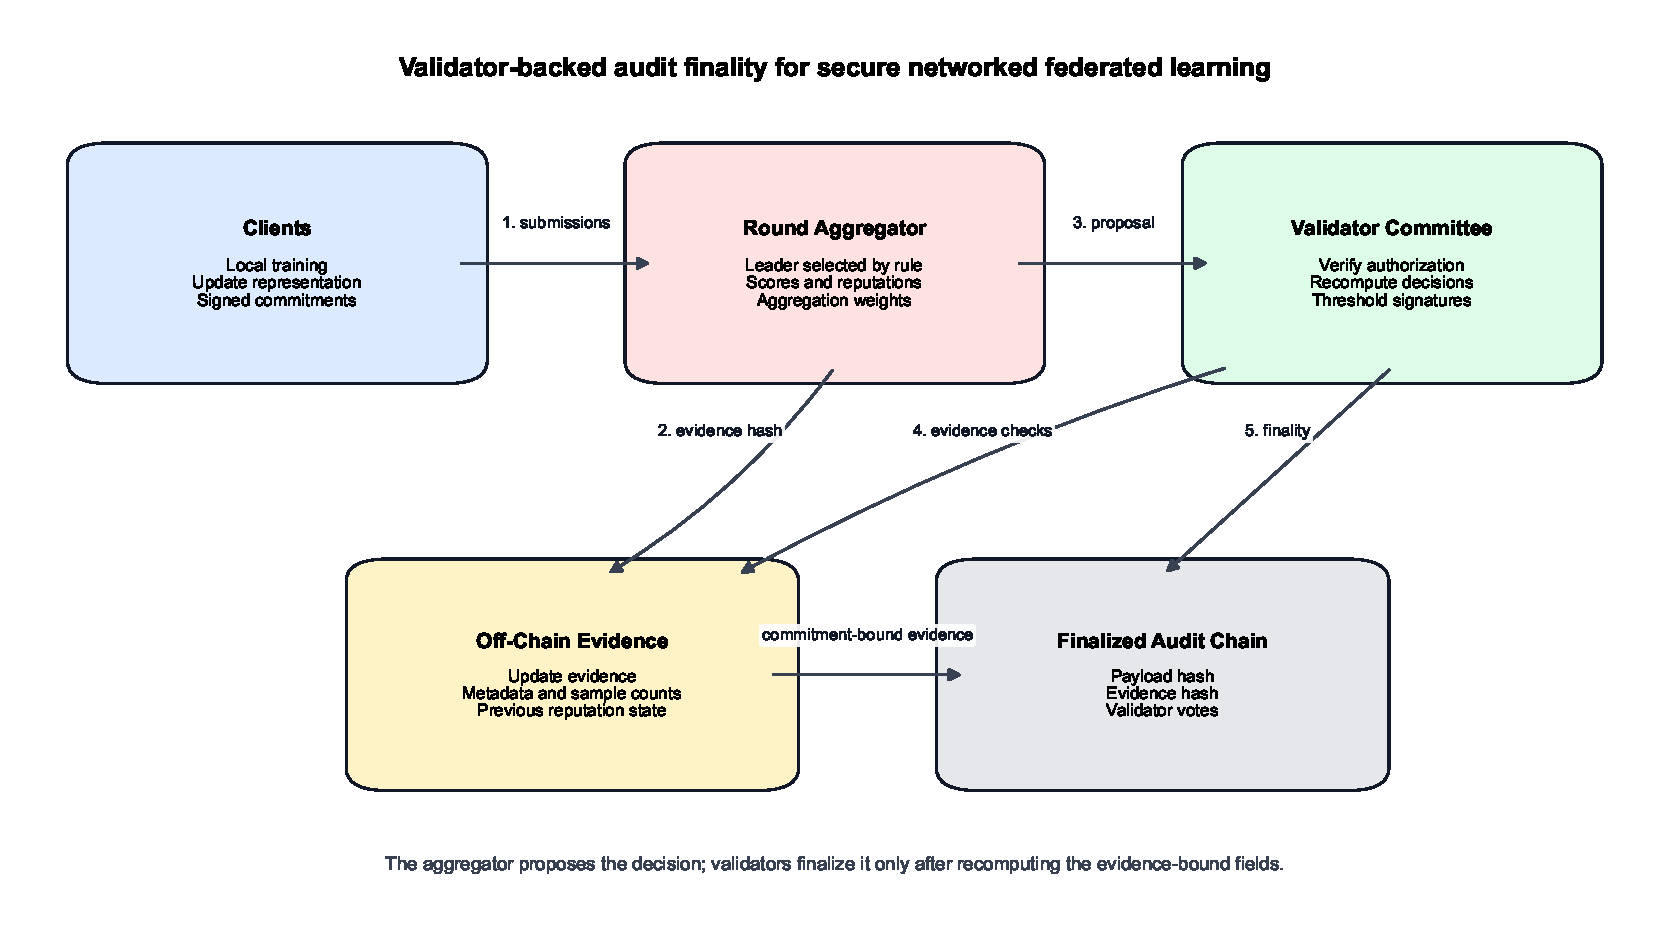
\includegraphics[width=\linewidth]{protocol_architecture.pdf}
\caption{Learning-system architecture of validator-backed auditable robust aggregation for trustworthy federated learning. The aggregator proposes anomaly scores, reputation updates, aggregation weights, and audit hashes; validators independently verify commitment-bound evidence before threshold finality.}
\label{fig:protocol-architecture}
\end{figure}

\subsection{Multi-Signal Anomaly Score}

For each round, the selected aggregator computes the update norm
\begin{equation}
r_{t,i}=\lVert u_{t,i}\rVert_2.
\end{equation}
The robust norm center is the median update norm:
\begin{equation}
c_t=\mathrm{median}_i(r_{t,i}).
\end{equation}
The robust scale is the median absolute deviation (MAD):
\begin{equation}
s_t=\max\{\mathrm{median}_i(|r_{t,i}-c_t|),\epsilon\},
\end{equation}
where $\epsilon$ is a small constant used to avoid division by zero. The one-sided norm anomaly score is
\begin{equation}
z^n_{t,i}=\max\left(0,\frac{r_{t,i}-c_t}{s_t}\right).
\end{equation}

The reference update direction is the mean update
\begin{equation}
\bar{u}_t=\frac{1}{N}\sum_i u_{t,i}.
\end{equation}
The directional consistency score uses cosine similarity:
\begin{equation}
d_{t,i}=\cos(u_{t,i},\bar{u}_t), \qquad
z^d_{t,i}=\max(0,1-d_{t,i}).
\end{equation}
If client $i$ participated in the previous round with stored update $u_{t-1,i}$, the history instability score is
\begin{equation}
z^h_{t,i}=\max(0,1-\cos(u_{t,i},u_{t-1,i})).
\end{equation}
For a new client without history, $z^h_{t,i}=0$. The final anomaly score is
\begin{equation}
A_{t,i}=0.45z^n_{t,i}+0.35z^d_{t,i}+0.20z^h_{t,i}.
\end{equation}
These coefficients are fixed across all main formal experiments. They encode the design priority that large magnitude deviations should receive the strongest immediate penalty, directional disagreement should remain a separate signal for adaptive and collusive updates, and history should stabilize repeated decisions without permanently excluding clients after one abnormal round. They are not tuned separately for Fashion-MNIST, CIFAR-10, or individual attacks. The sensitivity and ablation studies later test whether the method depends on one exact coefficient setting and whether each signal is necessary.

\subsection{Reputation and Client Commitments}

Each client has a reputation value $R_{t,i}$ initialized as $R_{0,i}=1$. After computing anomaly score $A_{t,i}$, reputation is updated by exponential smoothing:
\begin{equation}
R_{t+1,i}=\mathrm{clip}\left(0.85R_{t,i}+0.15\exp(-A_{t,i}),0.05,1.5\right).
\end{equation}
The clipping interval prevents permanent reputation collapse. It also bounds the maximum advantage of a client with consistently benign behavior.

Each client also signs a lightweight commitment containing round ID, client ID, update hash, sample count, and metadata hash. The commitment is not intended to reveal raw data or store full model updates on chain. Its purpose is to bind the off-chain evidence package to the finalized decision record, preventing a dishonest aggregator from inventing a client update, silently changing client metadata, or omitting submitted evidence without leaving a detectable mismatch between client commitments and the proposed audit payload. Validators therefore check both the commitment signatures and the availability of the referenced evidence needed to recompute the decision.

\subsection{Aggregator Proposal and Validator Finality}

Let $P_t$ denote the finalized round payload containing model hash, metrics, client metadata, anomaly scores, reputation values, aggregation weights, and client commitments. Let $E_t$ denote the off-chain round-evidence package containing the update vectors or equivalent verifiable update representation, sample counts, metadata, previous reputation state, previous-update references, and client signatures. The eligible aggregator for round $t$ is selected by a public deterministic rule in the current implementation:
\begin{equation}
g_t=\mathrm{sorted}(\mathcal{G})[(t-1)\bmod |\mathcal{G}|],
\end{equation}
where $\mathcal{G}$ is the permissioned aggregator set. The round-robin rule is used for reproducibility in the simulator. It can be replaced in deployment by a BFT leader-rotation rule, verifiable randomness, or a reputation-aware selection mechanism.

The selected aggregator signs a proposal containing the round number, aggregator ID, previous block hash, payload hash, evidence hash, and proposal hash. Validators then check: (i) the previous hash matches the latest finalized block; (ii) the payload hash, evidence hash, and proposal hash are correct; (iii) the aggregator is eligible for the round and its signature is valid; (iv) client commitments match the client records and signatures; (v) the client, decision, commitment, and evidence sets are consistent; and (vi) anomaly scores, rejection flags, reputation updates, and aggregation weights can be deterministically recomputed from $E_t$ and are consistent with the recorded decision evidence. A validator refuses to sign if required evidence is missing, if a commitment does not open to the referenced evidence, or if recomputation produces different scores or weights.

Each finalized audit block is
\begin{equation}
B_t=(t,\mathrm{timestamp}_t,h_{t-1},P_t), \qquad
h_t=\mathrm{SHA256}(\mathrm{canonical\_json}(B_t)).
\end{equation}
The next block stores $h_t$ as its previous hash. Verification checks both hash correctness and hash linkage from the genesis hash to the final block. In the validator-backed design, $B_t$ is finalized only after at least $q$ validators accept and sign the proposal.

The implemented audit layer is a permissioned threshold-finality simulation that models the audit component of a blockchain-assisted FL system. It does not implement full PBFT, HotStuff, Tendermint, or Fabric-style message flow, view change, networking, validator incentives, smart-contract execution, or gas accounting \citep{castro1999pbft,yin2019hotstuff,buchman2018tendermint,androulaki2018fabric}. This abstraction is deliberate: consensus protocols can order and finalize a submitted value, but they do not by themselves determine whether the FL-specific contents of that value are valid. If the application validity predicate accepts incorrect anomaly scores, reputation updates, aggregation weights, or model hashes, a full BFT system would only replicate agreement on an invalid FL decision. The experiment therefore isolates the scientific question of whether robust aggregation decisions can be made reconstructable and independently verifiable under client poisoning and aggregator-side tampering. The simulation should be read as an application-layer finality protocol for aggregation evidence, not as a claim of full blockchain-system performance. A production BFT or permissioned-ledger deployment would provide replicated ordering and finality for submitted proposals; it would still require the validity predicate evaluated here to decide whether a proposal's scores, weights, commitments, and model hashes are correct before validators sign it.

\subsection{Dynamic Weighted Aggregation}

The selected aggregator first applies hard-rejection rules. Client $i$ is hard rejected if any of the following conditions holds:
\begin{equation}
A_{t,i}>\tau_A,\qquad
z^n_{t,i}>\tau_n \ \mathrm{and}\ d_{t,i}<0,\qquad
d_{t,i}<\tau_d.
\end{equation}
The implemented default parameters are $\tau_A=4.0$, $\tau_n=2.5$, and $\tau_d=-0.4$. If a client is not hard rejected, its raw aggregation weight is
\begin{equation}
a_{t,i}=\max(a_{\min},R_{t+1,i}\exp(-\gamma A_{t,i})),
\end{equation}
where $a_{\min}=0$ and $\gamma=1.2$ in the formal experiments. If the hard-rejection condition is true, $a_{t,i}=0$. The final normalized aggregation coefficient is sample-size weighted according to Eq. (2). If all raw weights are zero, the implementation selects the lowest-anomaly 50\% of clients as a fallback set and assigns them exponentially decayed weights.

\subsection{Security and Audit Interpretation}

The proposed framework provides validator-backed decision traceability rather than a cryptographic proof that every malicious client is detected. For each round, the audit payload records the evidence used by the aggregation rule: update hashes, anomaly scores, reputation values before and after smoothing, hard-rejection flags, raw aggregation weights, normalized aggregation coefficients, and global evaluation metrics. Because the block hash is computed over a canonical representation of this payload and linked to the previous block hash, modifying a finalized past decision without recomputing and re-finalizing subsequent blocks changes the corresponding block hash and breaks the subsequent chain linkage. Because the proposal is finalized only with validator signatures, a single dishonest aggregator cannot unilaterally rewrite or finalize its own audit trail as long as the validator-threshold assumption holds.

The audit record supports four verification tasks. First, an auditor can recompute the hash chain to check whether the recorded training history has been modified. Second, given the stored round payload, the auditor can reconstruct why a client received zero, reduced, or full aggregation influence. Third, under the stated verification rules, validators can reject invalid proposals from unauthorized or dishonest aggregators before finality. Fourth, an auditor can inspect validator signatures and rejected votes to identify which validators approved or rejected a proposal. These checks are useful for accountability and forensic analysis, but they do not replace secure aggregation, differential privacy, trusted execution, full blockchain consensus, or permissionless identity management. Those mechanisms address different security goals and can be layered with the proposed aggregation logic in future deployments.

\subsection{Validator-Backed Audit Properties}

The validator-backed audit layer is designed to satisfy four audit properties under the threat model in Section 3. These properties are stated for the application-level validity predicate evaluated in this paper, not for a complete BFT networking stack.

\emph{Safety against unilateral aggregator tampering.} Let $\mathsf{Valid}(P_t,E_t,h_{t-1},g_t)$ denote the deterministic predicate that checks aggregator authorization, hash linkage, client commitments, evidence availability, score recomputation, reputation updates, rejection flags, aggregation weights, and proposal integrity. If fewer than $q$ validators sign proposals for which $\mathsf{Valid}=0$, then an invalid proposal cannot be finalized because finality requires at least $q$ accepting signatures. Therefore, a dishonest aggregator cannot unilaterally finalize altered scores, weights, client records, model hashes, or evidence hashes under the threshold assumption.

\emph{Liveness under validator availability.} If a valid proposal is broadcast to the committee, the evidence package is available, and at least $q$ validators are online and execute the verification predicate, then the proposal can obtain enough signatures for finality. If fewer than $q$ validators are available, the round may remain unfinalized even when the proposal is valid. The liveness claim is therefore conditional on validator availability, not on asynchronous-network progress guarantees.

\emph{Accountability for invalid signing.} Every finalized or attempted-finality record contains validator identities, signatures, accepted votes, and rejected votes. If a validator signs a proposal that later fails the public validity predicate, its signature links the validator identity to an invalid proposal hash. The protocol therefore produces objective evidence of invalid signing. In a permissioned consortium, this evidence can support governance actions such as temporary suspension, committee removal, validator-reputation reduction, or external contractual penalties. It does not by itself impose economic penalties or implement token-based slashing; those mechanisms belong to a deployment layer that can consume the recorded evidence.

\emph{Auditability and decision reconstructability.} For each finalized round, the stored payload and off-chain evidence references are sufficient to recompute anomaly scores, reputation updates, hard-rejection flags, raw aggregation weights, and normalized aggregation coefficients. An auditor can therefore reconstruct whether a client was accepted, down-weighted, rejected, or fallback selected in that round. This property concerns traceability of the recorded decision; it does not imply that the aggregation rule perfectly identifies every malicious client.

These properties explain the role of the validator committee. The committee is not introduced to make the learning algorithm more accurate. It prevents a single aggregation service from becoming the sole authority over both model aggregation and the audit trail, while making the security boundary explicit: threshold collusion can violate safety, and insufficient online validators can violate liveness. Committee sizing is therefore a security-performance trade-off. Larger committees and higher thresholds reduce the probability of threshold capture under random committee sampling, but increase proposal dissemination, local verification, and vote-collection costs. The protocol-cost, scalability, and latency experiments evaluate this trade-off for the application-layer validity predicate.

\subsection{Decision Semantics and Audit Evaluation Protocol}

The protocol follows three lines of prior work: Byzantine-robust aggregation evaluates whether malicious updates lose influence in the aggregate \citep{blanchard2017krum,yin2018byzantine,pillutla2022rfa}, trust-aware FL uses client-level evidence to weight or suppress suspicious participants \citep{cao2021fltrust,fung2020foolsgold}, and blockchain-assisted FL emphasizes tamper-resistant records and verifiable training histories \citep{lu2020blockchain,nguyen2021blockchainedge,dong2024blockchain,awan2022blockchainflsurvey}. Our audit protocol adapts these ideas to client-round decision tracing: it evaluates not only the final model utility but also whether the evidence behind each aggregation decision can be reproduced after training.

To make the audit interpretation explicit, each client-round decision is mapped to one of four states. A client is \emph{accepted} when it does not trigger a hard-rejection rule and receives a nonzero aggregation weight close to the benign-client range in that round. A client is \emph{down-weighted} when it does not trigger hard rejection but receives a reduced aggregation weight because its anomaly score increases or its reputation decreases. A client is \emph{rejected} when a hard-rejection rule sets $a_{t,i}=0$, meaning the client has no influence on the aggregate in that round. Finally, a client is \emph{fallback selected} only when all raw weights are zero and the lowest-anomaly clients are restored with small positive weights to avoid a stalled training round.

The explanation attached to a decision is not a free-form textual justification; it is a reconstructable record derived from the stored evidence. For each client and round, the audit payload stores the norm anomaly score, direction score, history score, combined anomaly score, reputation before and after updating, hard-rejection flag, raw aggregation weight, normalized aggregation coefficient, and fallback flag if applicable. Given these fields and the fixed thresholds in Table~\ref{tab:params}, an auditor can reproduce whether the client was accepted, down-weighted, rejected, or fallback selected, and can inspect which recorded signals contributed to the decision.

We evaluate auditability through four verification checks. First, \emph{chain validity} verifies that all block hashes and previous-hash links are intact. Second, \emph{decision reconstructability} checks whether the stored anomaly, reputation, threshold, and weight fields are sufficient to reproduce the recorded aggregation decision. Third, \emph{malicious influence suppression} is measured in controlled experiments by the mean aggregation weight and zero-weight rate assigned to known malicious clients. Fourth, \emph{benign retention} is inspected through nonzero aggregation weights for benign clients under Non-IID data. These metrics evaluate the traceability of aggregation decisions; they should not be interpreted as a guarantee that every malicious client is perfectly detected in deployment.

\begin{table}[t]
\centering
\caption{Proposed aggregation hyperparameters.}
\label{tab:params}
\resizebox{\linewidth}{!}{%
\begin{tabular}{lll}
\toprule
Parameter & Value & Meaning \\
\midrule
Norm coefficient & 0.45 & Norm-deviation weight in $A_{t,i}$ \\
Direction coefficient & 0.35 & Direction-inconsistency weight in $A_{t,i}$ \\
History coefficient & 0.20 & History-instability weight in $A_{t,i}$ \\
$\tau_A$ & 4.0 & Anomaly hard-rejection threshold \\
$\tau_n$ & 2.5 & Norm threshold used with negative direction \\
$\tau_d$ & -0.4 & Direction threshold for hard rejection \\
$\gamma$ & 1.2 & Exponential weight temperature \\
$a_{\min}$ & 0.0 & Minimum aggregation weight before fallback \\
Reputation clip & [0.05, 1.5] & Lower and upper reputation bounds \\
Fallback fraction & 0.5 & Lowest-anomaly fallback fraction \\
\bottomrule
\end{tabular}
}
\end{table}

\subsection{Algorithm}

\noindent\textbf{Algorithm 1: Validator-backed auditable robust aggregation.}
Given the current global model $w_t$, client models $\{w_{t,i}\}$, sample counts $\{n_i\}$, reputation table $\{R_{t,i}\}$, previous updates $\{u_{t-1,i}\}$, eligible aggregators $\mathcal{G}$, validator committee $\mathcal{V}$, threshold $q$, and previous finalized hash $h_{t-1}$:
\begin{enumerate}
  \item Each selected client submits a signed commitment over round ID, client ID, update hash, sample count, and metadata hash.
  \item Select the round aggregator $g_t$ using the public aggregator-selection rule.
  \item The aggregator computes update vectors $u_{t,i}$, norms $r_{t,i}$, median norm center $c_t$, MAD scale $s_t$, and mean update $\bar{u}_t$.
  \item The aggregator computes norm, direction, and history anomaly scores for each client.
  \item The aggregator updates reputation values $R_{t+1,i}$, computes hard-rejection decisions and aggregation weights $a_{t,i}$, and applies fallback selection if all raw weights are zero.
  \item The aggregator computes $w_{t+1}$ using sample-size-normalized weights and proposes an audit block containing hashes, metrics, anomaly evidence, reputation values, aggregation weights, rejection decisions, client commitments, evidence hash, and aggregator signature.
  \item Each validator verifies client commitments, aggregator eligibility, proposal signature, hash linkage, required decision fields, evidence availability, and deterministic recomputation of anomaly scores, reputation updates, rejection flags, and aggregation weights from the commitment-bound evidence.
  \item If at least $q$ validators accept and sign the proposal, finalize the audit block and set $h_t$ to the finalized block hash; otherwise the block remains unfinalized and the round requires recovery.
\end{enumerate}
The output is the updated global model, reputation table, previous-update cache, validator-signed audit block, and finalized audit hash.

\section{Experimental Setup}

\subsection{Evaluation Perspective}

The evaluation treats the framework as a trustworthy FL learning system rather than only as a model-aggregation heuristic. Learning experiments measure clean utility and attack resistance, while audit and validator experiments measure whether decision evidence is reconstructable, whether manipulated proposals are rejected before finality, whether invalid signing is attributable, and where validator availability or collusion changes the outcome. The overhead experiments further expose verification and finality costs, including message structure, proposal size, committee communication, local verification latency, bandwidth sensitivity, RTT sensitivity, and event-driven finality outcomes. This separation keeps model utility, application-level validity, and deployment cost visible as distinct evaluation dimensions.

\subsection{Datasets and Models}

MNIST is used for sanity checks, while Fashion-MNIST and CIFAR-10 serve as the main benchmarks. Fashion-MNIST is evaluated under both IID and Dirichlet Non-IID settings. CIFAR-10 is used to test whether the conclusions remain valid on a harder colored-image benchmark, with emphasis on the more challenging Non-IID setting. Because CIFAR-10 is substantially more expensive in the current FL simulator, we use it primarily as a three-seed Non-IID stress test rather than exhaustively repeating every IID setting.

\subsection{Data Distribution, Attacks, and Baselines}

The main Non-IID experiments use a Dirichlet split with $\alpha=0.5$. Each main setting uses 10 clients with a malicious ratio of 0.2 unless otherwise specified. The main attack set includes sign flipping, adaptive scaling, and backdoor trigger attacks. The implemented empirical baselines are FedAvg, Krum, Trimmed Mean, coordinate-wise Median, and norm filtering. These baselines cover unprotected averaging, distance-based selection, coordinate-wise robust statistics, and a strong norm-based filter.

We further include three extension studies to strengthen the security comparison. First, FLTrust is implemented as a trusted-root baseline using a small server-side root set of 100 samples to construct a reference update. This changes the trust model and is therefore reported separately from the main no-root-data baselines. Second, a FLAME-style backdoor baseline is implemented using cosine-distance clustering, norm clipping, and calibrated Gaussian noise. Because the project environment does not include HDBSCAN, this baseline should be interpreted as a FLAME-style implementation rather than a byte-for-byte reproduction of the original FLAME system. Third, we add a collusive-direction poisoning attack in which malicious clients coordinate an update direction against the benign mean while respecting adaptive norm constraints. This attack is intended to stress the decentralized-FL setting where attackers may coordinate rather than appear as independent outliers.

The trust assumption therefore differs across baselines. FLTrust assumes a trusted root dataset at the server side, FLAME-style defense targets backdoor mitigation through clustering and clipping, and classical robust aggregators assume the aggregation rule is executed faithfully. The proposed protocol instead assumes a permissioned validator committee with fewer than $q$ validators willing to sign invalid proposals and at least $q$ validators available for liveness. The experiments are designed to make these assumptions observable through invalid-proposal rejection, Byzantine-boundary, validator-accountability, and validator-dropout results.

\subsection{Metrics and Reproducibility}

The evaluation metrics include clean accuracy, best clean accuracy, test loss, attack success rate (ASR), rejection or zero-weight rate, chain validity, and runtime. Rejection-based metrics should be interpreted as aggregation decisions rather than perfect malicious-client detection labels. For auditability, we further report chain verification, simulated tamper detection, decision reconstruction, malicious suppression, benign retention, and benign--malicious aggregation-weight gap. For validator-backed finality, we report valid-block finalization, aggregator authorization checks, invalid-proposal rejection and acceptance, Byzantine-boundary behavior, invalid-signing rate, slashable validator identities, validator-dropout liveness, verification latency, and event-driven finalized/rejected/timeout outcomes. We also include a scalability sweep that expands recorded audit evidence to larger client and validator counts in order to measure proposal size, committee communication, and local verification latency. These metrics are computed from the recorded audit logs and protocol simulations rather than manually assigned after training.

All formal result tables are generated from the consolidated summary CSV using deterministic table-export scripts. The scripts keep the latest run for each experiment name and exclude smoke tests, tuning diagnostics, and extended exploratory attacks. Figures and audit-case materials are generated by the corresponding export scripts in the \texttt{experiments/} directory.

The validator-backed audit experiments are implemented as protocol simulations over recorded audit logs rather than as a full blockchain network. This choice isolates the application-level validity predicate: whether validators can independently reject manipulated aggregation evidence before finality. Network propagation, mempool ordering, view-change, validator admission, and economic incentives are important deployment issues, but including them would confound the evaluation of the aggregation-decision verification logic that is the focus of this study. This separation is necessary because consensus and application validity solve different problems. PBFT-, HotStuff-, Tendermint-, or Fabric-style protocols can make replicas agree on the same ordered value, but if the application predicate accepts incorrect anomaly scores or aggregation weights, the system may consistently finalize an invalid FL decision. The experiments therefore first test the FL-specific predicate that a full permissioned-ledger deployment would execute before signing or finalizing a block. Under the same validator evidence and threshold assumptions, the simulation exercises the same deterministic local proposal-validity checks that validators would run before signing and adds an event-driven finality model for proposal delivery, vote return, threshold outcomes, and timeout; it does not model full throughput, view-change behavior, validator membership, or incentive enforcement.

\section{Results and Discussion}

The results are reported in the order required by the paper's trustworthy-learning argument. We first establish poisoning robustness and clean-accuracy trade-offs, then test stronger extension baselines and coordinated poisoning, then isolate the proposed components through ablation, and finally evaluate whether recorded decisions are auditable and protected against unilateral aggregator tampering under the validator-threshold assumption. Auxiliary malicious-ratio, coefficient, runtime-overhead, and latency details are reported in the supplementary material so that the main text follows the central logic chain rather than treating every diagnostic check as a separate contribution. The claim-to-evidence mapping is explicit: Figures~\ref{fig:fashion-iid}--\ref{fig:proposed-norm-asr} and Supplementary Table S1 evaluate competitive robustness, Table~\ref{tab:collusive-extension} evaluates coordinated poisoning, Table~\ref{tab:ablation} tests component necessity, Tables~\ref{tab:audit-metrics}--\ref{tab:audit-multirun} evaluate decision reconstruction and traceability, Tables~\ref{tab:validator-tamper}--\ref{tab:validator-accountability} evaluate threshold-finality security boundaries, and Tables~\ref{tab:protocol-cost}, \ref{tab:validator-scalability}, and \ref{tab:network-events} evaluate verification cost, scalability, and event-driven finality behavior.

\begin{table}[t]
\centering
\caption{Claim-to-evidence map for the main evaluation claims.}
\label{tab:claim-evidence}
\small
\begin{tabular}{>{\raggedright\arraybackslash}p{0.26\linewidth}>{\raggedright\arraybackslash}p{0.34\linewidth}>{\raggedright\arraybackslash}p{0.30\linewidth}}
\toprule
Claim & Primary evidence & Scope boundary \\
\midrule
Competitive robustness under poisoning & Figures~\ref{fig:fashion-iid}--\ref{fig:proposed-norm-asr}, Supplementary Table S1 & Competitive, not accuracy-dominant in every setting \\
Coordinated-poisoning robustness & Table~\ref{tab:collusive-extension}, Table~\ref{tab:ablation} & Evaluated on Fashion-MNIST Non-IID collusive direction \\
Decision traceability & Tables~\ref{tab:audit-metrics}--\ref{tab:audit-multirun}, Supplementary Figures S2--S3 & Reconstructs recorded decisions, not perfect malicious-client detection \\
Aggregator-tamper resistance & Tables~\ref{tab:validator-tamper}--\ref{tab:validator-accountability} & Holds below the validator signing threshold \\
Verification cost and finality behavior & Tables~\ref{tab:protocol-cost}, \ref{tab:validator-scalability}, and \ref{tab:network-events}; Supplementary Tables S5--S6 & Measures validity-check cost and application-layer finality outcomes, not full BFT network throughput \\
\bottomrule
\end{tabular}
\end{table}

\subsection{Fashion-MNIST Main Results}

\begin{figure}[t]
\centering
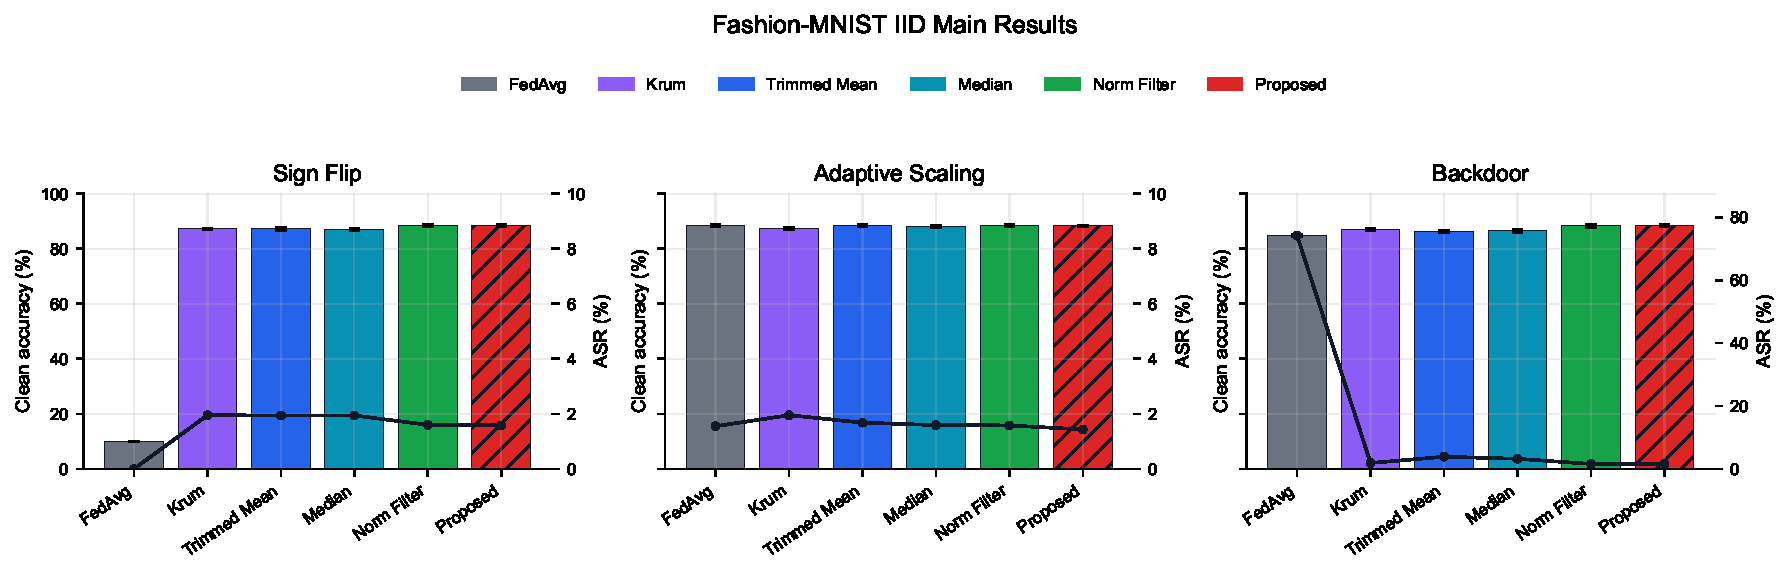
\includegraphics[width=\linewidth]{fashionmnist_iid_main.pdf}
\caption{Fashion-MNIST IID results. Bars show three-seed mean clean accuracy with standard-deviation error bars; the line shows ASR. Higher accuracy and lower ASR are better.}
\label{fig:fashion-iid}
\end{figure}

\begin{figure}[t]
\centering
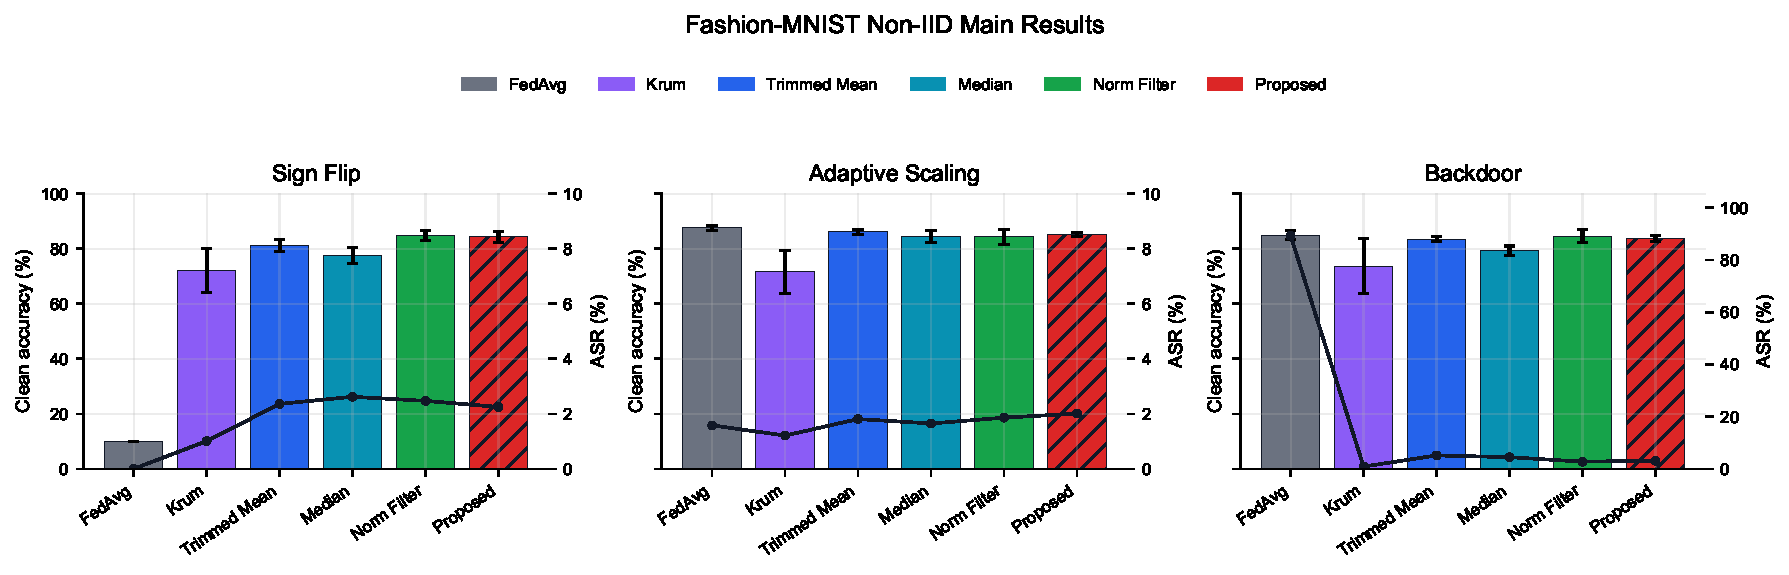
\includegraphics[width=\linewidth]{fashionmnist_noniid_main.pdf}
\caption{Fashion-MNIST Dirichlet Non-IID results. Bars show three-seed mean clean accuracy with standard-deviation error bars; the line shows ASR. Higher accuracy and lower ASR are better.}
\label{fig:fashion-noniid}
\end{figure}

On Fashion-MNIST, FedAvg collapses under sign flipping and remains vulnerable to backdoor attacks with high ASR. Krum avoids some attacks but suffers substantial clean-accuracy degradation under Non-IID data. The proposed method is stable across all Fashion-MNIST main settings. Under IID settings, it is essentially tied with norm filtering, reaching about 88.3\% clean accuracy with ASR around 1.4--1.6\%. Under Non-IID settings, it remains competitive, reaching 84.27\%, 85.21\%, and 83.67\% under sign flipping, adaptive scaling, and backdoor attacks. Trimmed Mean and norm filtering remain strong clean-accuracy competitors in some settings; the proposed method's advantage is therefore stable, auditable aggregation rather than guaranteed clean-accuracy dominance.

\subsection{CIFAR-10 Non-IID Results}

\begin{figure}[t]
\centering
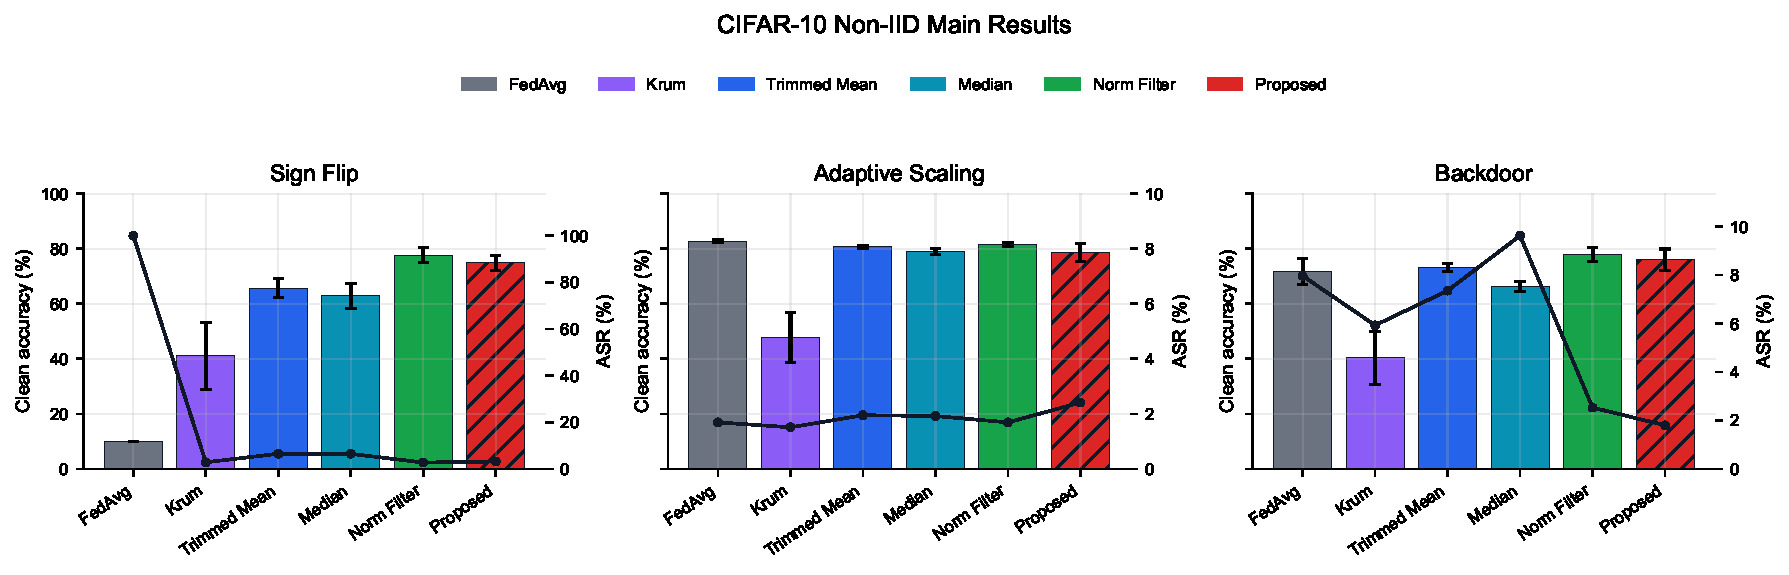
\includegraphics[width=\linewidth]{cifar10_noniid_main.pdf}
\caption{CIFAR-10 Dirichlet Non-IID results. Bars show three-seed mean clean accuracy with standard-deviation error bars; the line shows ASR. Higher accuracy and lower ASR are better.}
\label{fig:cifar-noniid}
\end{figure}

CIFAR-10 Non-IID provides a harder validation setting. FedAvg again collapses under sign flipping, and Krum shows large instability. Norm filtering is the strongest clean-accuracy baseline, reaching 77.62\%, 81.45\%, and 77.88\% under sign flipping, adaptive scaling, and backdoor attacks. The proposed method obtains 74.91\%, 78.61\%, and 76.04\%, respectively. Its ASR remains low, especially under backdoor attacks, but clean accuracy trails norm filtering by roughly 1.8--2.8 percentage points. These results support the paper's main claim precisely: the proposed method provides auditable, reputation-aware robustness with competitive accuracy and low ASR, while norm filtering is stronger when clean accuracy alone is the objective.

\begin{figure}[t]
\centering
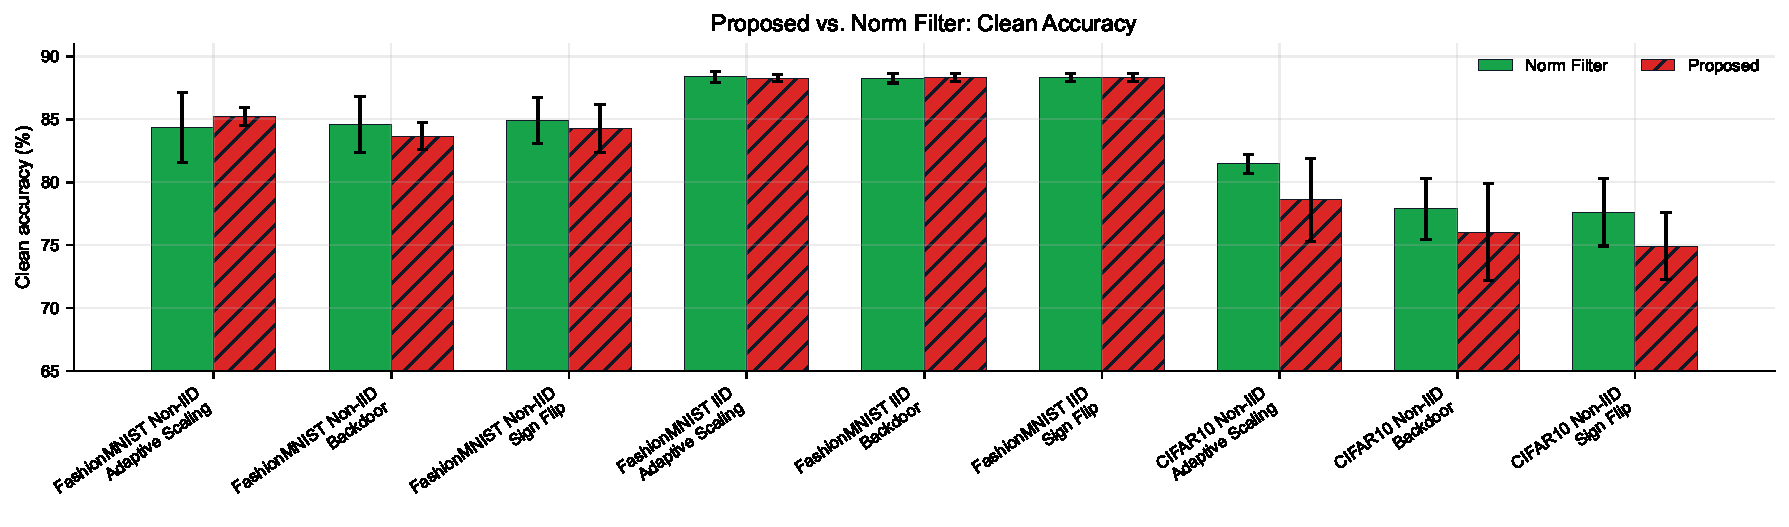
\includegraphics[width=\linewidth]{proposed_vs_norm_filter_accuracy.pdf}
\caption{Proposed vs. norm filtering clean accuracy across main benchmark conditions. Values are three-seed means; higher is better.}
\label{fig:proposed-norm-acc}
\end{figure}

\begin{figure}[t]
\centering
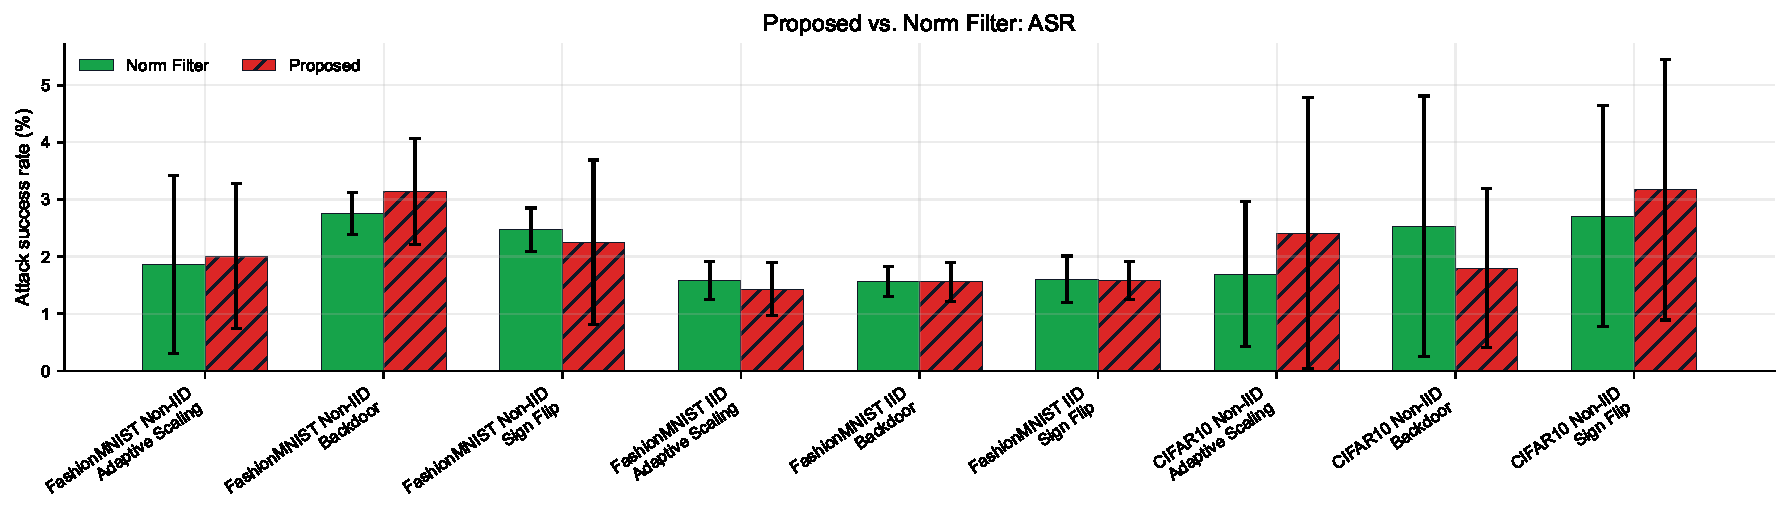
\includegraphics[width=\linewidth]{proposed_vs_norm_filter_asr.pdf}
\caption{Proposed vs. norm filtering ASR across main benchmark conditions. Values are three-seed means; lower is better.}
\label{fig:proposed-norm-asr}
\end{figure}

\subsection{Trusted-Root, Backdoor-Specific, and Collusive Extensions}

Supplementary Table S1 compares the proposed method with FLTrust and a FLAME-style backdoor defense under their stated assumptions. On Fashion-MNIST IID backdoor attacks, proposed and norm filtering both reach about 88.3\% clean accuracy and about 1.5\% ASR. On Fashion-MNIST Non-IID, proposed reaches 83.63\% accuracy and 3.17\% ASR, close to norm filtering at 84.59\% and 2.78\%. On CIFAR-10, norm filtering remains the strongest pure filtering baseline, while proposed closely matches ASR and trails slightly in clean accuracy. FLTrust and FLAME-style results show that trusted-root and clustering-based defenses are sensitive to their assumptions, data heterogeneity, and calibration.

Table~\ref{tab:collusive-extension} evaluates the DFL-specific collusive-direction attack on Fashion-MNIST Non-IID. Malicious clients coordinate a shared direction against the benign mean. The proposed method achieves the highest mean clean accuracy and the lowest accuracy standard deviation, while norm filtering has low ASR but suffers one seed-level collapse. This supports the use of directional consistency and reputation-aware weighting for coordinated poisoning.

\begin{table}[t]
\centering
\caption{Collusive-direction poisoning on Fashion-MNIST Non-IID. Values are mean $\pm$ standard deviation over three seeds; higher accuracy and lower ASR/loss are better.}
\label{tab:collusive-extension}
\resizebox{0.86\linewidth}{!}{%
\begin{tabular}{lrrrr}
\toprule
Method & Clean accuracy & Best accuracy & ASR & Loss \\
\midrule
FedAvg & 76.45 $\pm$ 7.85 & 76.45 & 2.82 $\pm$ 0.16 & 0.6694 \\
FLTrust & 64.68 $\pm$ 4.05 & 64.72 & 3.76 $\pm$ 1.74 & 1.1466 \\
Norm Filter & 44.84 $\pm$ 30.88 & 62.98 & 0.88 $\pm$ 1.53 & 108985.1528 \\
Proposed & 82.68 $\pm$ 2.26 & 84.46 & 2.02 $\pm$ 1.10 & 0.4558 \\
\bottomrule
\end{tabular}}
\end{table}

\subsection{Auxiliary Sensitivity Checks}

The auxiliary sensitivity analyses are used to check whether the main robustness conclusions depend on one narrow operating point. Supplementary Figure S1 reports Fashion-MNIST Non-IID adaptive-scaling results at malicious ratios of 10\%, 20\%, and 40\%. Proposed, Trimmed Mean, and norm filtering all remain stable with no early stopping; the proposed method maintains approximately 85.0--85.2\% clean accuracy and about 2.0\% ASR across the three ratios, while Trimmed Mean has the best average clean accuracy in this particular setting. Supplementary Table S2 evaluates anomaly-score coefficient variants under sign-flip and adaptive-scaling attacks. All variants complete without early stopping, and most remain close to the default configuration. Supplementary Table S7 further varies the malicious ratio under collusive-direction poisoning. Proposed remains competitive at 10\% and is the strongest method at 20\%, but all evaluated methods collapse near random accuracy at 40\%, which identifies a high-adversary-fraction boundary rather than a universal robustness claim. These checks support stability under representative parameter and adversary-strength shifts, but they are reported as diagnostic evidence rather than as independent contributions.

\subsection{Ablation Study}

Table~\ref{tab:ablation} evaluates three components of the proposed aggregation rule on Fashion-MNIST Non-IID: direction scoring, history scoring, and hard rejection. The backdoor ablation shows that several variants can keep ASR low, indicating that the backdoor setting is not dominated by a single component. The collusive-direction attack is more diagnostic. Removing direction scoring reduces mean clean accuracy from 82.80\% to 77.47\%, and removing hard rejection reduces it to 78.12\%. Removing history scoring has a smaller effect on the mean but increases the accuracy standard deviation from 1.09 to 3.09. These results support the design choice of combining instantaneous directional evidence, hard suppression of highly suspicious updates, and temporal reputation evidence. Direction and hard rejection are especially important for coordinated directional poisoning, while history contributes mainly to stability across seeds.

\begin{table}[t]
\centering
\caption{Proposed-method ablation on Fashion-MNIST Non-IID. Values are mean $\pm$ standard deviation over three seeds; higher accuracy and lower ASR/loss are better.}
\label{tab:ablation}
\resizebox{\linewidth}{!}{%
\begin{tabular}{llrrrr}
\toprule
Attack & Variant & Clean accuracy & Best accuracy & ASR & Loss \\
\midrule
Backdoor & Full & 83.68 $\pm$ 1.08 & 84.15 & 3.18 $\pm$ 0.90 & 0.4263 \\
Backdoor & No direction & 83.85 $\pm$ 1.33 & 83.98 & 1.92 $\pm$ 1.19 & 0.4287 \\
Backdoor & No hard rejection & 83.79 $\pm$ 0.94 & 84.31 & 2.96 $\pm$ 0.72 & 0.4225 \\
Backdoor & No history & 83.25 $\pm$ 0.74 & 83.54 & 2.80 $\pm$ 0.63 & 0.4330 \\
\midrule
Collusive direction & Full & 82.80 $\pm$ 1.09 & 84.49 & 1.97 $\pm$ 0.87 & 0.4428 \\
Collusive direction & No direction & 77.47 $\pm$ 1.93 & 77.75 & 3.05 $\pm$ 0.44 & 0.6139 \\
Collusive direction & No hard rejection & 78.12 $\pm$ 1.51 & 78.44 & 3.04 $\pm$ 0.15 & 0.5626 \\
Collusive direction & No history & 81.36 $\pm$ 3.09 & 83.92 & 1.63 $\pm$ 1.24 & 0.4635 \\
\bottomrule
\end{tabular}}
\end{table}

\subsection{Auditability}

For every completed run, the framework records per-round metrics, per-client aggregation decisions, and hash-linked audit evidence. In the validator-backed protocol simulation, these records become finalized only after validator verification and threshold signing. This audit trail is the main system-level distinction from ordinary robust aggregation baselines. The paper emphasizes auditability and reproducible decision tracing as first-class design goals, while clean accuracy and ASR demonstrate that the audit mechanism is paired with a practically competitive defense.

A representative audit case uses Fashion-MNIST Non-IID sign-flip attack with the proposed method and seed 42. The run contains 80 audit blocks and passes hash-linkage verification, satisfying the chain-validity check. The stored per-client fields also support decision reconstruction because each zero-weight or reduced-weight decision can be traced to the recorded anomaly scores, reputation values, rejection flags, and aggregation weights. The final clean accuracy is 86.47\%, the best clean accuracy is 86.47\%, and the final ASR is 1.08\%. The two malicious clients receive zero mean aggregation weight across all 80 rounds, while benign clients retain an average aggregation weight of 0.2831. This case demonstrates malicious influence suppression and benign retention in the controlled benchmark, while also showing how the recorded evidence supports post-hoc inspection of aggregation decisions.

Table~\ref{tab:audit-metrics} quantifies this auditability claim. Chain verification succeeds for the recorded audit chain, and a simulated tamper test detects all single-block modifications of recorded metrics. The decision reconstruction rate is 100\%, meaning that all 800 client-round aggregation decisions in the case can be reproduced from the stored decision fields. Malicious client-rounds receive zero aggregation weight in all cases, while 85.78\% of benign client-rounds retain nonzero contribution. The mean rejection precision is lower than recall because several benign Non-IID clients are conservatively assigned zero weight in some rounds. This confirms that the rejection signal should be interpreted as a cautious aggregation decision rather than a perfect malicious-client detector.

\begin{table}[t]
\centering
\caption{Auditability and client-influence metrics for the representative audit case. Higher chain verification, tamper detection, decision reconstruction, malicious suppression, and benign retention are better; rejection precision/recall describes zero-weight decisions, not perfect malicious-client detection.}
\label{tab:audit-metrics}
\resizebox{\linewidth}{!}{%
\begin{tabular}{llp{7.5cm}}
\toprule
Metric & Value & Interpretation \\
\midrule
Stored audit blocks & 80 & Number of hash-linked round records. \\
Chain verification rate & 100.00\% & Recorded hashes and previous-hash links are valid. \\
Tamper detection rate & 100.00\% & All simulated single-block metric modifications are detected. \\
Decision reconstruction rate & 100.00\% & All 800 client-round decisions are reproducible from stored decision fields. \\
Malicious suppression rate & 100.00\% & Malicious client-rounds receive zero aggregation weight. \\
Benign retention rate & 85.78\% & Benign client-rounds retain nonzero aggregation weight. \\
Benign--malicious weight gap & 0.2831 & Difference between mean benign and malicious aggregation weights. \\
Mean rejection precision / recall & 64.38\% / 100.00\% & Zero-weight decisions suppress all malicious client-rounds but also conservatively reject some benign Non-IID updates. \\
\bottomrule
\end{tabular}}
\end{table}

To verify that these auditability properties are not limited to one selected case, we also compute the same objective audit metrics across all latest formal proposed-method runs after removing superseded duplicate runs. This multi-run audit evaluation covers the main benchmark settings and the malicious-ratio sensitivity study. As shown in Table~\ref{tab:audit-multirun}, all 39 proposed-method runs pass chain verification, simulated tamper detection, and decision reconstruction. In total, the audit logs contain 3600 hash-linked blocks and 36000 client-round decisions. Benign retention remains high on average, but it varies across attacks and data heterogeneity because the defense sometimes assigns zero weight to benign Non-IID clients conservatively. This is why rejection-related metrics are reported as aggregation-decision statistics rather than as perfect detection metrics.

\begin{table}[t]
\centering
\caption{Multi-run auditability summary for latest formal proposed-method runs. Values are mean $\pm$ standard deviation over runs; higher audit rates are better.}
\label{tab:audit-multirun}
\resizebox{\linewidth}{!}{%
\begin{tabular}{lrrrr}
\toprule
Scope & Runs / blocks / decisions & Chain verification & Tamper detection & Decision reconstruction / benign retention \\
\midrule
Main benchmark & 30 / 2880 / 28800 & 100.00 $\pm$ 0.00\% & 100.00 $\pm$ 0.00\% & 100.00 $\pm$ 0.00\% / 95.56 $\pm$ 6.48\% \\
Malicious-ratio sensitivity & 9 / 720 / 7200 & 100.00 $\pm$ 0.00\% & 100.00 $\pm$ 0.00\% & 100.00 $\pm$ 0.00\% / 100.00 $\pm$ 0.00\% \\
All proposed runs & 39 / 3600 / 36000 & 100.00 $\pm$ 0.00\% & 100.00 $\pm$ 0.00\% & 100.00 $\pm$ 0.00\% / 96.59 $\pm$ 5.97\% \\
\bottomrule
\end{tabular}}
\end{table}

Supplementary Figures S2--S3 provide the corresponding single-run trajectory and per-client weight visualization for the representative audit case. They are placed in the supplementary material because the main claim is supported by the objective reconstruction and tamper-detection metrics in Tables~\ref{tab:audit-metrics}--\ref{tab:audit-multirun}, while the figures serve as interpretive examples.

\subsection{Validator-Backed Finality Under Aggregator Tampering}

The preceding audit metrics evaluate whether recorded aggregation decisions can be reconstructed after training. We next evaluate whether a dishonest aggregator can finalize manipulated audit evidence. The validator-backed protocol is tested on the latest 39 formal proposed-method runs, covering 3600 valid audit blocks. For each valid block, we generate invalid proposals by tampering with score fields, aggregation weights, client records, model hashes, previous hashes, client signatures, payload hashes, evidence hashes, missing evidence packages, self-consistent score or weight edits that recompute proposal hashes, aggregator authorization, aggregator signatures, and equivocation-style proposal content.

Table~\ref{tab:validator-tamper} summarizes the protocol-security result. Valid proposals finalize in all cases, while all tested invalid proposals are rejected before finality. The invalid-proposal acceptance rate is 0\% under the default honest-validator setting. This result addresses the core security distinction between a single-server hash chain and validator-backed audit finality: the aggregator can propose a decision, but it cannot unilaterally finalize a manipulated evidence record without validator-threshold approval.

The strongest tampering cases are the self-consistent score and weight edits: after modifying recorded decision fields, the simulated dishonest aggregator recomputes proposal hashes and aggregator signatures. These proposals are still rejected because validators recompute the deterministic decision fields from the commitment-bound evidence rather than accepting a hash-consistent proposal at face value.

\begin{table}[t]
\centering
\caption{Validator-backed finality under aggregator and payload tampering. Values summarize 39 proposed-method runs and 3600 valid audit blocks; higher valid finalization/rejection and lower invalid acceptance are better.}
\label{tab:validator-tamper}
\resizebox{\linewidth}{!}{%
\begin{tabular}{lrrrrr}
\toprule
Scenario group & Runs & Tampered blocks & Valid finalization & Invalid rejection & Invalid acceptance \\
\midrule
Score/weight/payload/evidence tampering & 39 & 50400 & 100.00\% & 100.00\% & 0.00\% \\
Aggregator authorization/signature/equivocation tampering & 39 & 10800 & 100.00\% & 100.00\% & 0.00\% \\
All invalid proposals & 39 & 61200 & 100.00\% & 100.00\% & 0.00\% \\
\bottomrule
\end{tabular}}
\end{table}

Threshold finality is not unconditional. It depends on the number of validators that are honest and available. Table~\ref{tab:byzantine-boundary} reports the Byzantine-validator boundary. With five validators and threshold three, invalid proposals are rejected when zero, one, or two validators are Byzantine, but accepted when three Byzantine validators reach the signing threshold. With seven validators and threshold five, the same boundary appears when five Byzantine validators sign invalid proposals. This table is intentionally reported because it makes the trust assumption explicit: the protocol prevents unilateral aggregator manipulation, but it cannot withstand a signing threshold of colluding validators.

\begin{table}[t]
\centering
\caption{Byzantine-validator boundary for threshold finality. Values are means over 13 representative runs; higher invalid acceptance indicates threshold compromise.}
\label{tab:byzantine-boundary}
\resizebox{\linewidth}{!}{%
\begin{tabular}{rrrrrr}
\toprule
Validators & Threshold & Byzantine validators & Valid finalization & Invalid rejection & Invalid acceptance \\
\midrule
5 & 3 & 0 & 100.00\% & 100.00\% & 0.00\% \\
5 & 3 & 1 & 100.00\% & 100.00\% & 0.00\% \\
5 & 3 & 2 & 100.00\% & 100.00\% & 0.00\% \\
5 & 3 & 3 & 100.00\% & 0.00\% & 100.00\% \\
7 & 5 & 2 & 100.00\% & 100.00\% & 0.00\% \\
7 & 5 & 4 & 100.00\% & 100.00\% & 0.00\% \\
7 & 5 & 5 & 100.00\% & 0.00\% & 100.00\% \\
\bottomrule
\end{tabular}}
\end{table}

Supplementary Table S3 reports the corresponding liveness boundary under validator dropout. Valid blocks continue to finalize as long as the number of online validators reaches the threshold; once the available validator count falls below threshold, valid-block finalization fails. This is a liveness failure rather than a poisoning-defense failure, and it clarifies the availability assumption required by the committee design.

The same threshold-signature records also provide accountability evidence. Table~\ref{tab:validator-accountability} reports invalid-signing rates under several validator-fault settings. When the committee is honest, no validator signs invalid proposals. When Byzantine validators are present but remain below the finality threshold, invalid proposals are not finalized, but the validators that signed them are still identifiable. For example, with five validators and threshold three, two Byzantine validators generate an invalid-signing rate of 40\% over invalid proposals but an invalid-finalization rate of 0\%; the two signing validators are slashable from the recorded evidence. Once Byzantine signers reach the threshold, invalid-finalization becomes possible, and the signed evidence identifies the colluding validator set. This does not implement a full economic slashing mechanism, but it converts validator misbehavior into objective evidence that a permissioned consortium can use for punishment, removal, or reputation updates.

\begin{table}[t]
\centering
\caption{Validator accountability under invalid proposal signing. Values are computed over 13 representative runs; invalid signing and slashable validators quantify accountability evidence.}
\label{tab:validator-accountability}
\resizebox{\linewidth}{!}{%
\begin{tabular}{rrrrrr}
\toprule
Validators & Threshold & Byzantine validators & Invalid signing rate & Invalid finalization & Slashable validators \\
\midrule
5 & 3 & 0 & 0.00\% & 0.00\% & 0 \\
5 & 3 & 2 & 40.00\% & 0.00\% & 2 \\
5 & 3 & 3 & 60.00\% & 100.00\% & 3 \\
7 & 5 & 4 & 57.14\% & 0.00\% & 4 \\
7 & 5 & 5 & 71.43\% & 100.00\% & 5 \\
\bottomrule
\end{tabular}}
\end{table}

\subsection{Runtime and Audit Overhead}

\begin{table}[t]
\centering
\caption{Per-round verification and audit cost of the validator-backed audit layer. $N$ is the number of participating clients, $m$ is the validator committee size, $q$ is the signing threshold, $S_u$ is the update representation size, $S_c$ is the client commitment size, and $S_p$ is the compact proposal/audit-payload size.}
\label{tab:protocol-cost}
\resizebox{\linewidth}{!}{%
\begin{tabular}{llll}
\toprule
Stage & Messages / operations & Main transmitted or checked data & Scaling \\
\midrule
Client submission & $N$ client uploads & Update representation, sample count, metadata, commitment & $O(N(S_u+S_c))$ \\
Aggregator proposal & One proposal to validators & Payload hash, evidence hash, model hash, scores, weights, signature & $O(mS_p)$ \\
Validator verification & $m$ local checks & Commitments, evidence availability, score/weight recomputation, hash linkage & $O(mN)$ checks \\
Threshold finality & At least $q$ validator signatures & Accept/reject votes and threshold-signed audit block & $O(m)$ votes, $q$ signatures \\
Audit storage & One finalized block & Compact decision evidence and hashes, not raw training data & $O(N)$ per round \\
\bottomrule
\end{tabular}}
\end{table}

Table~\ref{tab:protocol-cost} summarizes the per-round communication and verification structure introduced by the validator-backed audit layer. The design adds one aggregator-to-committee proposal phase and one committee finality phase beyond ordinary server-mediated FL. The dominant transmitted object remains the client update representation or its verifiable off-chain equivalent; the finalized audit chain stores compact decision evidence and hashes rather than raw training data. The local verification work scales with the number of validators and clients because each validator recomputes the deterministic score and weight fields from the commitment-bound evidence.

The proposed method records more per-client information than ordinary robust aggregation baselines, so its audit log is larger, but the measured runtime overhead is moderate in the current implementation. Supplementary Table S5 reports the detailed per-round timing and audit-log sizes. On Fashion-MNIST, the proposed method averages 1.788 s per round, compared with 1.434 s for norm filtering. On CIFAR-10, the proposed method averages 18.719 s per round, close to norm filtering at 18.550 s. The average defense computation time is small relative to total round time. These results indicate that, in the evaluated implementation, the main cost of the proposed approach is richer audit logging rather than a large increase in aggregation computation.

Validator verification also remains lightweight in the protocol simulation. In the recorded 10-client formal audit logs, valid proposal verification takes approximately 1.3--1.6 ms per block in the default setting with five validators and threshold three, and increasing the committee size to seven validators raises verification time to approximately 1.8--2.3 ms per block. The synthetic scalability sweep below is intentionally more demanding because it expands the number of client-evidence rows. These measurements cover local cryptographic checks, commitment verification, evidence availability checks, deterministic score/weight recomputation, proposal consistency checks, and threshold-finality simulation; they do not include real network propagation, mempool ordering, view-change, or smart-contract execution.

Table~\ref{tab:validator-scalability} reports a validator-side scalability sweep using recorded audit evidence expanded to larger client counts. The purpose of this experiment is not to create new model-training utility results, but to measure how the validator-backed validity predicate scales when the number of client evidence rows and validators increases. The default committee setting $(m,q)=(5,3)$ verifies 10, 50, 100, and 200-client proposals in approximately 2.05 ms, 9.12 ms, 18.04 ms, and 35.13 ms, respectively. With 100 synthetic client-evidence rows, increasing the committee from $(3,2)$ to $(11,7)$ raises verification time from 10.81 ms to 39.25 ms. In the reported sweep, valid proposals finalize and self-consistent weight-tampering proposals are rejected in 100\% of evaluated blocks. The proposal size grows roughly linearly with the client count because client commitments and decision evidence are included for each participant; committee communication scales with the number of validators because the proposal is sent to each validator.

\begin{table}[t]
\centering
\caption{Validator-side scalability of audit verification. Client counts are obtained by deterministic expansion of recorded audit evidence; rejection is measured against self-consistent weight tampering.}
\label{tab:validator-scalability}
\resizebox{\linewidth}{!}{%
\begin{tabular}{rrrrrrr}
\toprule
Clients & Validators & Threshold & Proposal KB & Committee KB/round & Valid verification ms & Invalid rejection \\
\midrule
10 & 5 & 3 & 12.55 & 62.73 & 2.05 & 100\% \\
50 & 5 & 3 & 56.91 & 284.54 & 9.12 & 100\% \\
100 & 5 & 3 & 112.36 & 561.82 & 18.04 & 100\% \\
200 & 5 & 3 & 223.66 & 1118.32 & 35.13 & 100\% \\
100 & 3 & 2 & 112.36 & 337.09 & 10.81 & 100\% \\
100 & 7 & 4 & 112.36 & 786.54 & 25.08 & 100\% \\
100 & 9 & 6 & 112.36 & 1011.27 & 32.29 & 100\% \\
100 & 11 & 7 & 112.36 & 1236.00 & 39.25 & 100\% \\
\bottomrule
\end{tabular}%
}
\end{table}

Supplementary Table S6 estimates finality latency under representative network conditions using the measured proposal sizes and validator verification times from Table~\ref{tab:validator-scalability}. The model assumes one aggregator-to-validator proposal phase and one validator-to-aggregator vote/finality phase, so estimated latency is $2\mathrm{RTT}$ plus proposal transmission time, vote-record transmission time, and local validator verification time. Under a 100 Mbps link and 10 ms RTT, the estimated finality latency remains below 75 ms for the 200-client, five-validator setting. Under a slower 10 Mbps link and 50 ms RTT, the same 200-client setting rises to about 319 ms. These results indicate that RTT dominates wide-area deployments, while proposal size becomes important for larger client populations and lower-bandwidth links.

We further run an event-driven finality simulation to separate network delay from threshold behavior. Each trial simulates proposal delivery to validators, local verification, vote return, threshold finalization or rejection, and timeout under deterministic pseudo-random propagation jitter and independent validator dropout. The simulation uses the measured proposal sizes and verification costs from Table~\ref{tab:validator-scalability}; it is still a permissioned application-layer finality model rather than a full PBFT, HotStuff, or Tendermint implementation. Table~\ref{tab:network-events} shows that valid proposals finalize reliably when the committee is available, invalid proposals are rejected when enough honest validators can reach the threshold, and invalid acceptance occurs only when Byzantine signers reach the signing threshold. The 11-validator case with six Byzantine validators is informative: invalid proposals are not accepted, but the five remaining honest validators cannot reach the seven-signature rejection threshold, so the outcome is timeout rather than finalization. This makes the safety and liveness boundary more explicit than the analytical latency estimate alone.

\begin{table}[t]
\centering
\caption{Event-driven validator-finality simulation. The network column reports bandwidth/RTT; rates are percentages over 500 trials. Higher valid finalization and invalid rejection are better; lower invalid acceptance and timeout are better.}
\label{tab:network-events}
\resizebox{\linewidth}{!}{%
\begin{tabular}{rrrrlrlrrrr}
\toprule
Clients & Validators & Threshold & Byzantine & Proposal & Dropout & Network & Finalized & Rejected & Invalid accepted & Timeout \\
\midrule
100 & 5 & 3 & 0 & Valid & 0\% & 100 Mbps / 10 ms & 100.00\% & 0.00\% & 0.00\% & 0.00\% \\
200 & 5 & 3 & 0 & Valid & 0\% & 100 Mbps / 10 ms & 100.00\% & 0.00\% & 0.00\% & 0.00\% \\
200 & 5 & 3 & 0 & Valid & 20\% & 100 Mbps / 10 ms & 92.40\% & 0.00\% & 0.00\% & 7.60\% \\
200 & 5 & 3 & 2 & Invalid & 0\% & 100 Mbps / 10 ms & 0.00\% & 100.00\% & 0.00\% & 0.00\% \\
200 & 5 & 3 & 3 & Invalid & 0\% & 100 Mbps / 10 ms & 0.00\% & 0.00\% & 100.00\% & 0.00\% \\
200 & 11 & 7 & 0 & Valid & 0\% & 10 Mbps / 100 ms & 100.00\% & 0.00\% & 0.00\% & 0.00\% \\
200 & 11 & 7 & 6 & Invalid & 0\% & 10 Mbps / 100 ms & 0.00\% & 0.00\% & 0.00\% & 100.00\% \\
200 & 11 & 7 & 7 & Invalid & 0\% & 10 Mbps / 100 ms & 0.00\% & 0.00\% & 100.00\% & 0.00\% \\
\bottomrule
\end{tabular}%
}
\end{table}

\subsection{Implications for Secure Federated Learning}

The empirical results should be read as a validation of the paper's security chain rather than as a single accuracy ranking. Main benchmarks, malicious-ratio tests, FLTrust and FLAME-style extensions, and the collusive-direction stress test show that the proposed method avoids the FedAvg failure modes observed in the attacked settings, keeps ASR low, and remains competitive with strong filtering baselines in the evaluated settings. The ablation study explains why the recorded norm, direction, history, reputation, and hard-rejection signals are not merely metadata: direction scoring and hard rejection are important under coordinated poisoning, while history information improves seed-level stability.

The audit-finality results address the central server objection directly. Robust aggregation reduces immediate malicious influence, while validator-backed auditability preserves and verifies the evidence needed to explain, reproduce, and challenge aggregation decisions after training. This matters in multi-organization deployments where down-weighting or exclusion can affect future participation and trust. The validator experiments show that a single aggregator cannot finalize manipulated evidence under the threshold assumption, invalid signing is attributable, and liveness depends on sufficient validator availability. The overhead, latency, and event-driven finality analyses indicate that this traceability is feasible in the evaluated simulator, but they should not be read as full end-to-end blockchain performance measurements.

\section{Limitations and Future Work}

The current experiments support auditable and robustly competitive aggregation, but the scope boundaries are explicit. The method is not optimized for clean accuracy alone: norm filtering is particularly strong on CIFAR-10, and Trimmed Mean performs best in the Fashion-MNIST adaptive-scaling malicious-ratio sensitivity experiment. Under collusive-direction poisoning, the proposed method is competitive at 10\% malicious participation and strongest at 20\%, but all evaluated methods collapse near random accuracy at 40\%, indicating a high-adversary-fraction boundary rather than universal robustness. The FLTrust and FLAME-style extensions improve baseline coverage, but they are reported under their stated assumptions rather than as definitive reimplementations of every prior defense. The coefficient study covers representative shifts, not a full hyperparameter surface. The scalability sweep expands recorded decision evidence to measure validator-side cost and is not a new 200-client utility-training study. The network-latency and event-driven finality analyses do not include packet loss, retransmission, queueing, mempool ordering, leader view changes, or complete BFT consensus networking.

The validator model also has security limits. A signing threshold of colluding or lazy validators can finalize invalid proposals, although their signatures provide accountability evidence. If fewer than $q$ validators are online, valid blocks cannot finalize. The current design assumes permissioned validator identities and reports slashable evidence, but does not implement permissionless Sybil resistance, on-chain slashing, stake economics, randomized committee sampling, or adaptive validator reputation. It also assumes that validators can access enough commitment-bound evidence to recompute score and weight fields; privacy-preserving robust validation under secure aggregation is outside the current implementation. Future work should improve CIFAR-10 clean accuracy without sacrificing auditability, evaluate additional defenses with official implementations, extend sensitivity analysis to larger models and thresholds, integrate privacy-preserving validity checks such as verifiable secure aggregation or zero-knowledge score verification, and embed the validity predicate into a realistic permissioned-ledger deployment.

\section{Conclusion}

This paper presents a permissioned validator-backed auditable robust aggregation framework for trustworthy federated learning under poisoning attacks and aggregator-side tampering. The framework combines multi-signal anomaly scoring, reputation-aware weighting, client commitments, rotating aggregator proposals, and threshold validator finality. It makes aggregation decisions reconstructable while preventing a single aggregator from unilaterally finalizing manipulated audit evidence under explicit committee assumptions. The experiments show that the method avoids the FedAvg failure modes observed in the attacked settings, maintains low ASR, and remains competitive with strong filtering baselines in the evaluated settings. FLTrust and FLAME-style extensions clarify how the proposed method compares with trusted-root and backdoor-specific defenses, while collusive-direction and ablation results show that direction scoring and hard rejection are important under coordinated poisoning and that very high malicious participation remains a boundary case. Validator experiments show that tested invalid proposals are rejected under the validator-threshold assumption, invalid-signing validators are identifiable, liveness depends on sufficient validator availability, and event-driven finality outcomes follow the stated threshold boundary. The contribution should therefore be understood as auditable and competitive robust aggregation for trustworthy FL with explicit validator-backed security boundaries rather than universal clean-accuracy dominance or a complete production blockchain deployment.

\section{Declarations}

\subsection{Data and Code Availability}

The experiments use public image benchmark datasets: MNIST, Fashion-MNIST, and CIFAR-10. The project repository provides the experimental scripts, generated manifests, consolidated summary tables, paper figures, audit-case excerpts, and audit-derived protocol tables used to reproduce the reported analyses. Formal result tables are generated from the consolidated summary CSV using deterministic export scripts, and the audit case study is generated from recorded per-round and per-client logs. The full raw run directories are not redistributed in the compact repository package but can be regenerated by running the released manifests. A cleaned reproducibility package containing the paper-specific code, configurations, and analysis scripts is available at \url{https://github.com/shiqiexperience/validator-backed-auditable-robust-fl}; the archived release is available on Zenodo at \url{https://doi.org/10.5281/zenodo.20790584}.

\subsection{Author Contributions}

Shiqi Huang: Conceptualization, methodology, software, validation, formal analysis, investigation, data curation, writing--original draft, writing--review and editing, visualization, and project administration.

\subsection{Funding}

This research did not receive any specific grant from funding agencies in the public, commercial, or not-for-profit sectors.

\subsection{Declaration of Competing Interest}

The author declares that there are no known competing financial interests or personal relationships that could have appeared to influence the work reported in this paper.

\subsection{Ethics and Security Scope}

This study uses public benchmark datasets and does not involve human subjects or private client data. The threat model focuses on poisoning robustness, aggregator-side tampering, validator-backed finality, and reconstructable aggregation decisions in federated learning. Privacy leakage, secure aggregation protocols, permissionless Sybil resistance, full adversarial consensus networking, smart-contract vulnerabilities, and economic incentive attacks are outside the scope of the current implementation and should be evaluated separately in a full deployment study.

\subsection{Declaration of Generative AI and AI-Assisted Technologies}

During the preparation of this work, the author used OpenAI ChatGPT/Codex to support manuscript organization, language editing, consistency checking, and preparation of submission materials. After using these tools, the author reviewed and edited the content as needed and takes full responsibility for the content of the article.

\bibliographystyle{elsarticle-num}
\bibliography{references}

\end{document}
